\chapter{Modeling of Train Operations}
\label{chap:ModelingOfTrainOperations}
\par\noindent
\emph{\textbf{Introduction}} As has been noted in \ref{sec:Solution}, it is necessary to model the braking process of freight trains. All modeling work has been performed with Matlab Simulink. 

\section{Initial Model}
\label{sec:InitialModel}
\par\noindent
The initial model to be expanded upon describes a single braking process. Let's take a look at the whole model first. 

\begin{figure}[H]
	\centering
	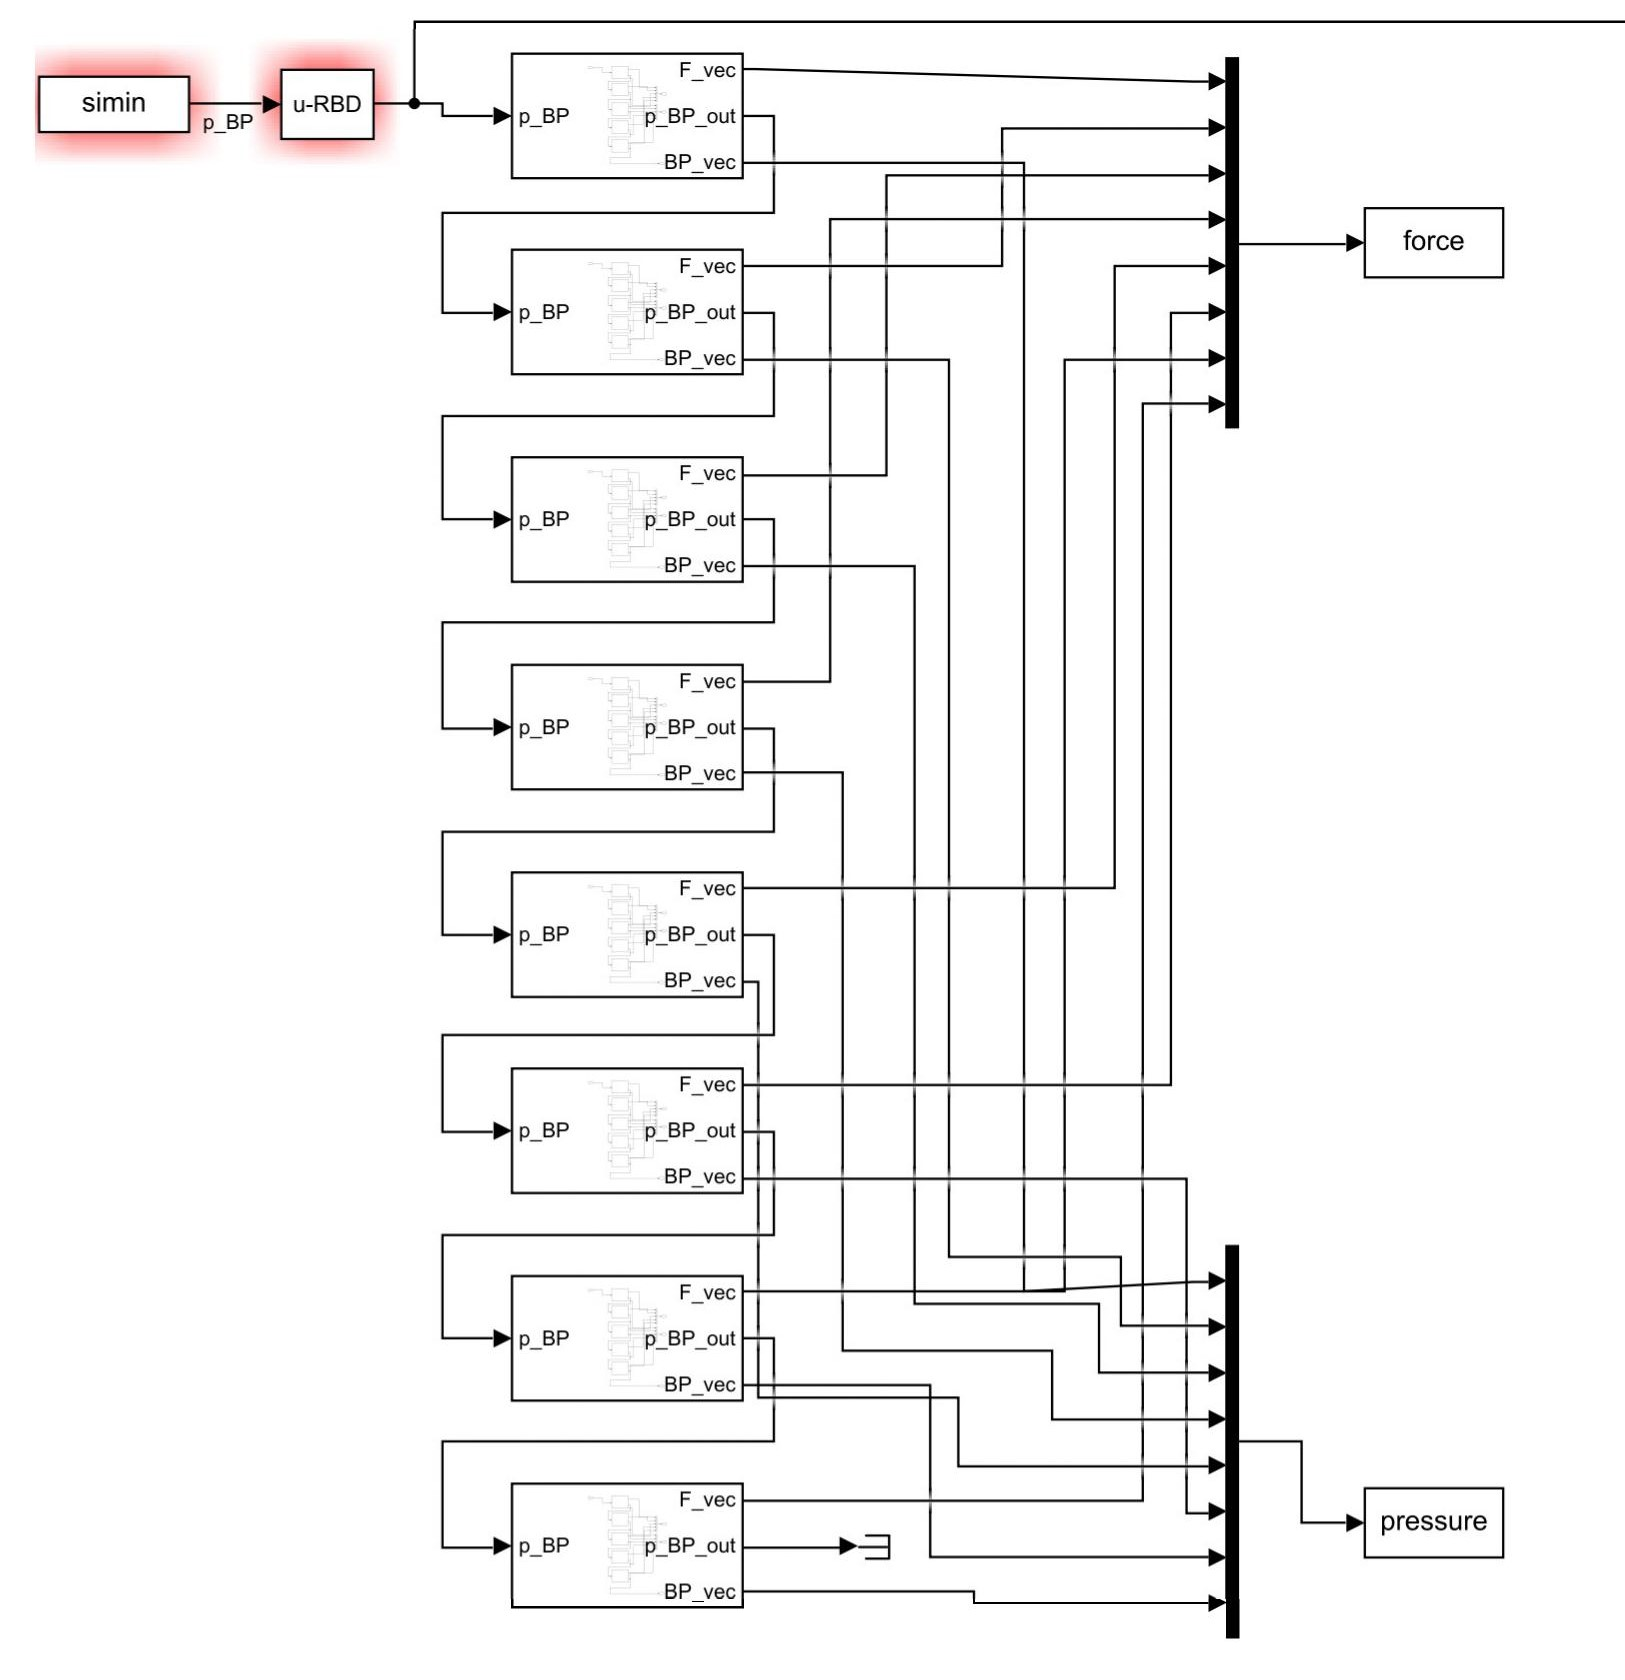
\includegraphics[width=\linewidth]{./pic/initmodel_whole}
	\caption{Initial model}
	\label{fig:initmodel_whole}
\end{figure}

\par\noindent
Here we see a model of a freight train of fixed length, consisting of 40 wagons, which are, for better readability, further condensed to subsystems of five wagons each, so there are eight of these subsystems. They are interconnected via braking pipe, which is also the sole input to each system. Outputs are braking pressure and braking force. We will take a look at the actual wagon model next.

\begin{figure}[H]
	\centering
	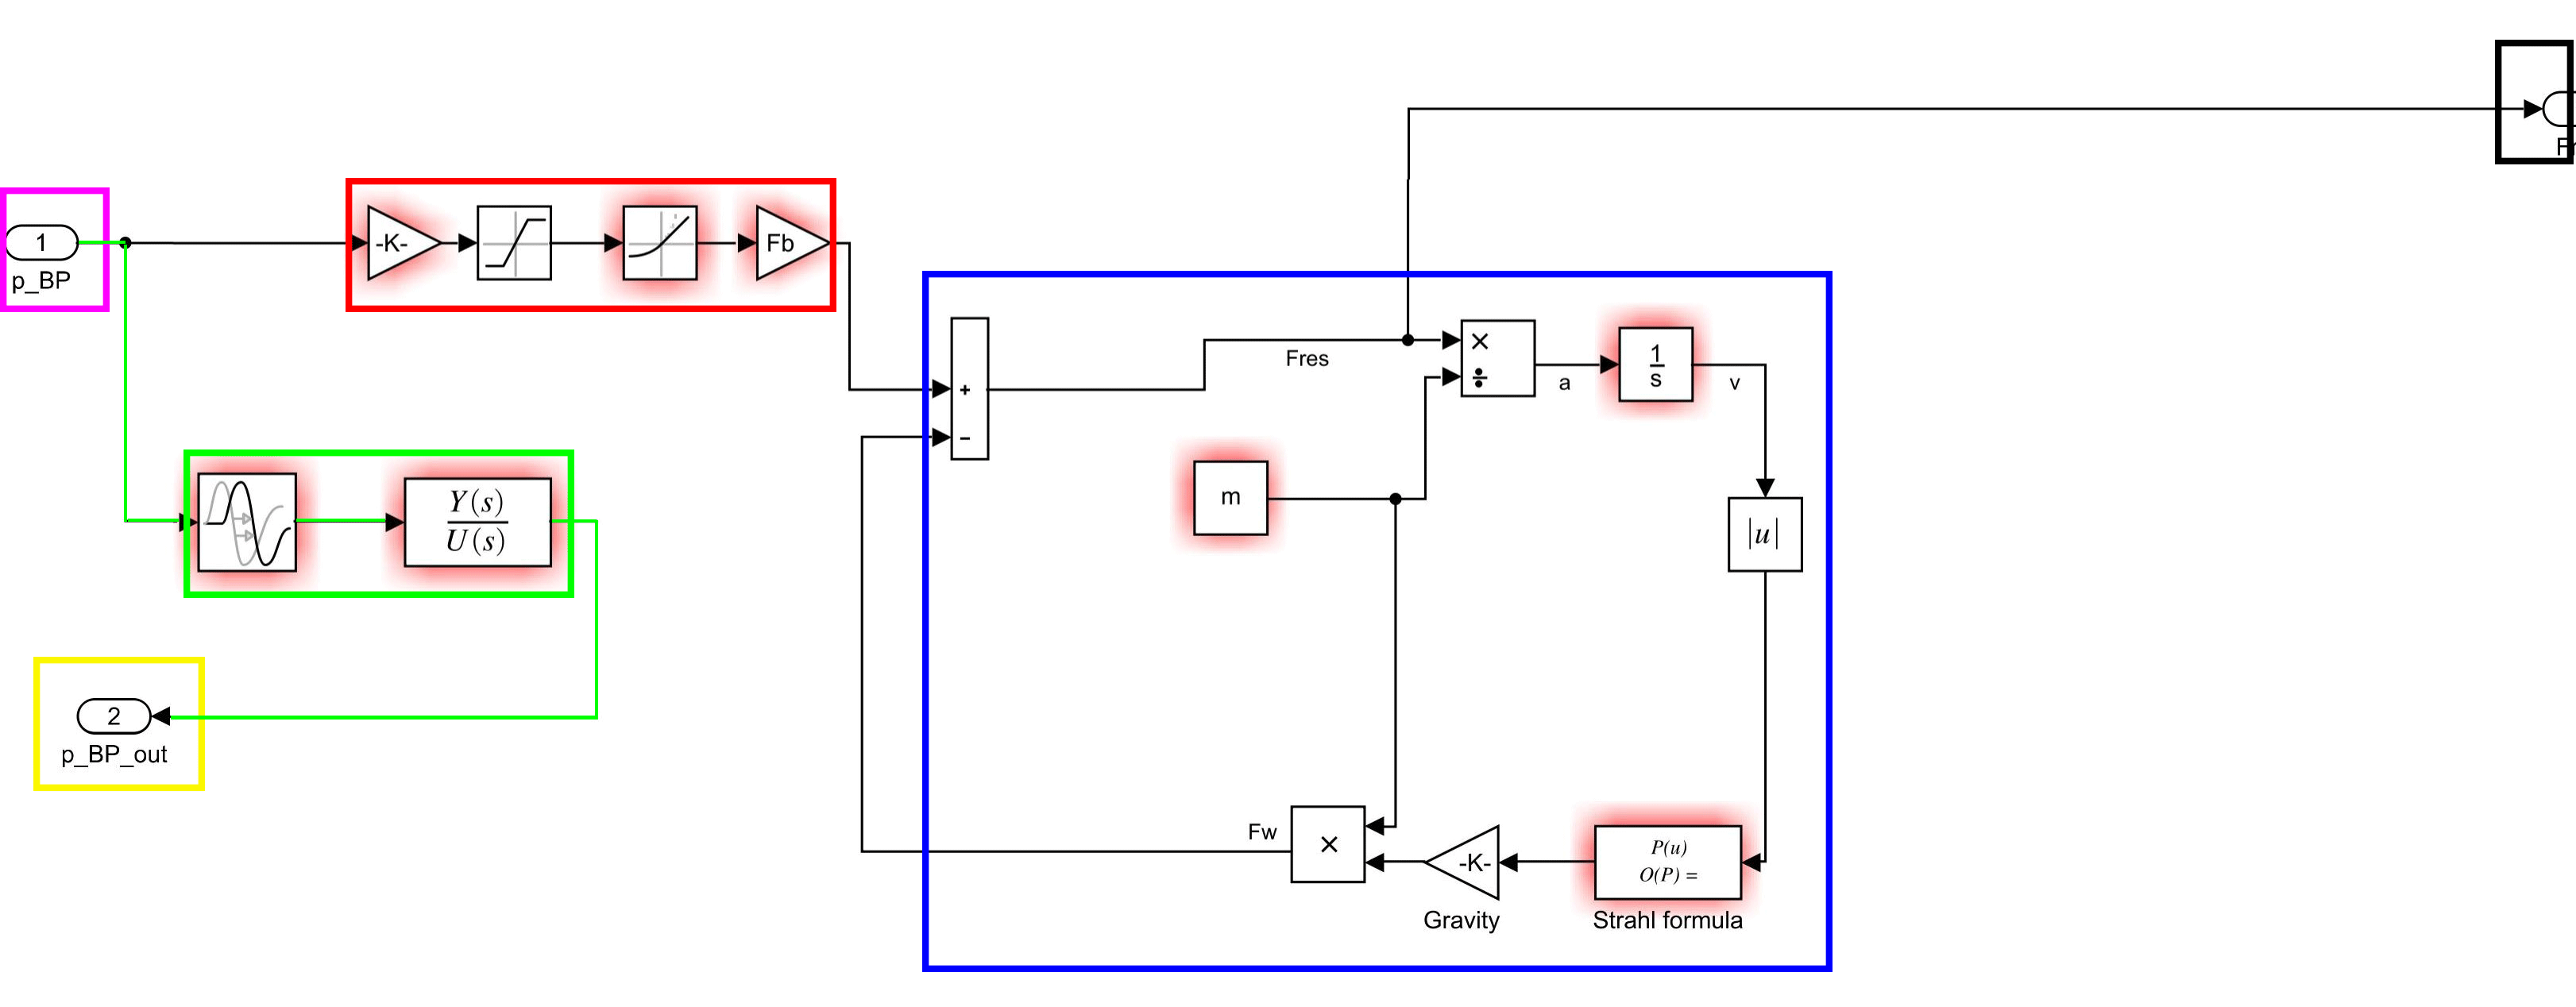
\includegraphics[width=\linewidth]{./pic/initmodel_wagon}
	\caption{Initial model - Wagon}
	\label{fig:initmodel_wagon}
\end{figure}

\par\noindent
Above is the initial wagon model. \NOTE{All 40 wagon models are identical here. This will be addressed in section \ref{sec:ModelExpansion}}. It consists of three main components.
\par
In the upper left corner is the input, which is the current pressure in the braking pipe. In the lower left corner, the propagation delay of the braking pipe is calculated. This is done by \TODO{}. Top center describes the calculation of the actual braking force, which is achieved by \TODO{}. Finally, the \TODO{Formulieren: Fahrzeugwiderstand}.

\section{Model Expansion}
\label{sec:ModelExpansion}

\section{Further Expansion}
\label{sec:FurtherExpansion}